

\chapter{Inleiding}
Het doel van dit OGO project is het maken van een UV waferstepper.
Een waferstepper is een machine die silicium wafers belicht om er
IC's van te maken. Omdat de details op de wafers zo klein zijn dat
normaal licht een te grote golflengte heeft, wordt UV licht
gebruikt. Dit UV licht heeft echter als nadeel dat ze door de
atmosfeer geabsorbeerd wordt. Daarom gebeurt het belichten van de
wafers in een vacu\"um. Bovendien gaan de lenzen die gebruikt worden
bij het belichten stuk wanneer ze aan de buitenlucht worden
blootgesteld.


De waferstepper die wij gaan maken, moet er als volgt uit komen te
zien.

\begin{figure}[!h]
\begin{center}
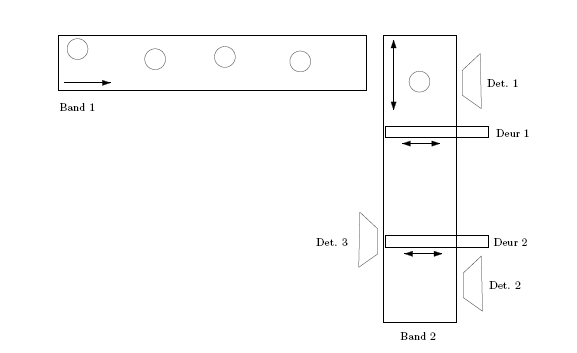
\includegraphics[width=0.8\linewidth]{schets}
\end{center}
\caption{Schema van de waferstepper}
\label{fig:schema}
\end{figure}

De belichtingsunit van de waferstepper is bereikbaar via een sluis
met twee deuren. Deze deuren mogen n\'{o}\'{o}it tegelijkertijd open
staan. Er zijn twee lopende banden. E\'{e}n waar te verwerken wafers
klaar liggen, deze kan maar \'{e}\'{e}n richting op, en \'{e}\'{e}n
waarop steeds een wafer door de deuren naar de belichtingsunit gaat
en weer terug. Wanneer een wafer bij de belichtingsunit komt, wordt
de band stilgezet, zodat de wafer belicht kan worden. Dit belichten
duurt precies twee seconden. Daarna gaat de wafer via de sluisdeuren
naar de verzamelbak.

Er bevinden zich twee licht detectoren in het systeem om de wafers
te lokaliseren. Deze detectoren bevinden zich aan de uiteinden van
de tweede band. Als er een wafer van de tweede band afvalt of af
wordt gehaald, dan wordt dit aangegeven door een extra led op het
processorbord te laten branden. Als er zo vijf wafers verloren gaan,
stopt het systeem en kan het alleen gerestart worden door een reset.

De wafers worden handmatig op de eerste band gelegd. Er is een
drukknop om aan te geven dat er wafers klaarliggen. Ook is er een
noodknop om het systeem te stoppen, en daarna weer te hervatten.

De waferstepper moet ten alle tijde aan de volgende voorwaarden
voldoen:
\begin{itemize}
  \item Wanneer de noodknop wordt ingedrukt stopt het systeem
  resoluut. Als de noodknop nu opnieuw wordt ingedrukt, hervat het
  systeem zijn oude taken, behalve als op zo'n moment een wafer belicht werd.
  Deze wafer is dan namelijk mislukt en zal niet opnieuw belicht worden.
  \item Beide sluisdeuren mogen nooit tegelijkertijd open staan,
  want dit zou de lens onherstelbaar beschadigen. Als een deur
  weigert te sluiten en dit gedetecteerd wordt door de sensor bij de
  deur, mag de andere deur dus niet opengaan.
  \item Wanneer er op de eerste band wafers klaar liggen en de ready
  button is ingedrukt, worden alle wafers zo snel mogelijk verwerkt en in de bak
  afgeleverd. Tenzij een wafer van de band valt. Het aantal van de band
  gevallen wafers komt overeen met het aantal brandende ledjes op het processorbord.
\end{itemize}
Verder geldt als algemeen design principe dat motoren,
luchtschakelaars en verlichting niet onnodig aangezet worden.

We maken eerst een systeemontwerp en bouwen de waferstepper. Hierna
maken we een programmaontwerp in UPPAAL. Met de Systeemanalyse
controleren we of het programmaontwerp goed werkt. Ten slotte
implementeren we het programmaontwerp in assembly, zodat we een
werkende waferstepper krijgen.
